\section{Einbinden von Grafiken}
\begin{frame}[c]
	\begin{center}
		\LARGE \textbf{Einbinden von Grafiken}
	\end{center}
\end{frame}
%%-----------------------------------------------------------------------------------------------%
%%------------------------------------------SUBSECTION-------------------------------------------%
%%-----------------------------------------------------------------------------------------------%
\subsection{Grundlagen}
\begin{frame}[c]
	\begin{center}
		\large Grundlagen
	\end{center}
\end{frame}
%-----------------------------------------------------------------------------------%
%---------------------------------------FRAME---------------------------------------%
%-----------------------------------------------------------------------------------%
\begin{frame}[fragile]
	\Ausgabe
	\begin{outputbox}
		\begin{figure}
			\centering
			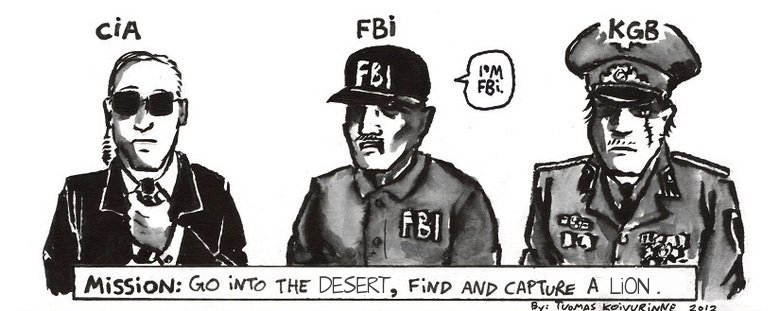
\includegraphics[width=0.3\textwidth]{img/loewenjagd}
		\end{figure}
	\end{outputbox}

	\pause\Code
	\begin{lstlisting}
\begin{figure}
	\centering
	\includegraphics[]{meinbild.jpg}
\end{figure}
	\end{lstlisting}

	\pause\textbf{Dateitypen:}\vspace{-0.2cm}
	\begin{itemize}
		\item *.pdf
		\item *.png
		\item *.eps
		\item *.jpg
	\end{itemize}
\note[item]<1>{1}
\note[item]<1>{1}
\note[item]<2>{2}
\end{frame}
%-----------------------------------------------------------------------------------%
%---------------------------------------FRAME---------------------------------------%
%-----------------------------------------------------------------------------------%
\begin{frame}[fragile]
	\begin{Aufgabe}
		Füge einen neuen Abschnitt \textrm{\qquote{Diktatorische Methode}} als \lstinline[basicstyle=\normalfont\ttfamily\normalsize]|\subsubsection| der Section \textrm{\qquote{Sonstige Methoden}} ein und schreibe folgenden Text:
		
		\textrm{\qquote{Man fange was man finde und prügele es so lange, bis es zugibt, ein Löwe zu sein, der in der Wüste gefangen wurde.}}
		
		Füge dann danach die Grafik \qquote{loewenjagd.png} mithilfe von \lstinline[basicstyle=\normalfont\ttfamily\normalsize]|\begin{figure}...\end{figure}|, \lstinline[basicstyle=\normalfont\ttfamily\normalsize]|\centering| und \lstinline[basicstyle=\normalfont\ttfamily\normalsize]|\includegraphics[]{}| ein.
	\end{Aufgabe}

	\btVFill\Befehle
	\begin{center}
		\begin{tabular}{ll}
			\toprule
			\LaTeX\ Befehl								&	Funktion								\\ \midrule
			\lstinline|\includegraphics[]{}|			&	Befehl zum Einbinden von Grafiken		\\ 
			\lstinline|\centering|						&	Zentrierung								\\
			\lstinline|\begin{figure}...\end{figure}|	&	Umgebung für Abbildungen				\\
			\lstinline|\caption{}|						&	Text der Bild Unter- oder Überschrift	\\
			\lstinline|\textwidth|						&	Gibt die Breite des Textbereichs aus	\\
			\bottomrule
		\end{tabular}
	\end{center}
\end{frame}
%-----------------------------------------------------------------------------------%
%---------------------------------------FRAME---------------------------------------%
%-----------------------------------------------------------------------------------%
\begin{frame}[fragile]
	\Losung
	\begin{outputbox}
		{\Large \textbf{2.3 Sonstige Methoden}}
		
		{\large \textbf{2.3.1  Diktatorische Methode}}
		
		Man fange was man finde und prügele es so lange, bis es zugibt, ein Löwe zu sein, der in der Wüste gefangen wurde.
		\vspace{-0.2cm}
		\begin{figure}[H]
			\centering
			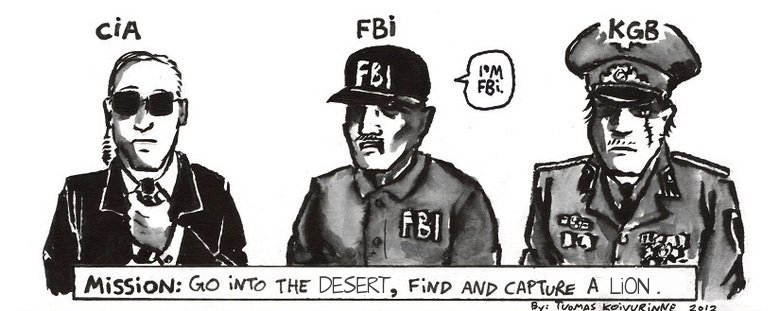
\includegraphics[width=0.2\textwidth]{img/loewenjagd.png}
		\end{figure}
		\vspace{-0.2cm}
	\end{outputbox}
	
	\Code
	\begin{lstlisting}
\subsection{Sonstige Methoden}
	\subsubsection{Diktatorische Methode}
		Man fange was man finde und prügele es so lange, bis es zugibt, ein Löwe zu sein, der in der Wüste gefangen wurde.
		\begin{figure}
			\centering
			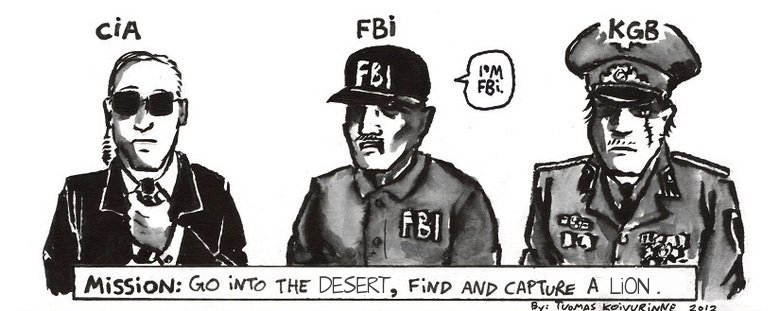
\includegraphics[]{img/loewenjagd.png}
		\end{figure}
	\end{lstlisting}
\end{frame}
%%-----------------------------------------------------------------------------------------------%
%%------------------------------------------SUBSECTION-------------------------------------------%
%%-----------------------------------------------------------------------------------------------%
\subsection{Einstellen der Größe}
\begin{frame}[c]
	\begin{center}
		\large Einstellen der Größe
	\end{center}
\end{frame}
%-----------------------------------------------------------------------------------%
%---------------------------------------FRAME---------------------------------------%
%-----------------------------------------------------------------------------------%
\begin{frame}[fragile]
	\begin{lstlisting}
\includegraphics[width=0.2\textwidth]{meinbild.jpg}
	\end{lstlisting}
	\pause
	\begin{outputbox}
		\begin{figure}[H]
			\centering
			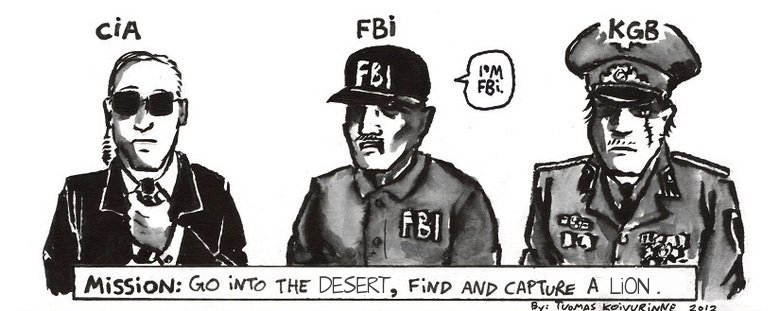
\includegraphics[width=0.2\textwidth]{img/loewenjagd.png}
		\end{figure}
	\end{outputbox}
	
	\pause
	\begin{lstlisting}
\includegraphics[width=0.4\textwidth]{meinbild.jpg}
	\end{lstlisting}
	\pause
	\begin{outputbox}
		\begin{figure}[H]
			\centering
			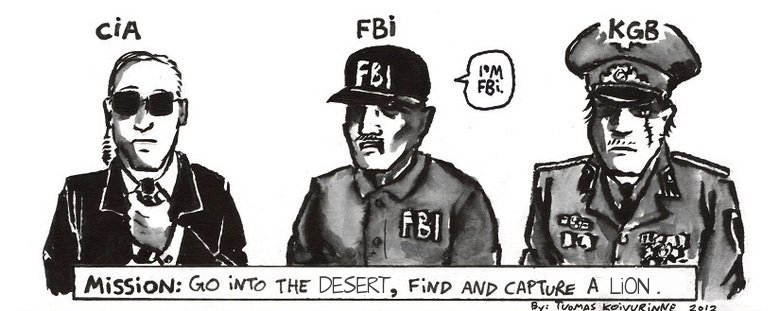
\includegraphics[width=0.5\textwidth]{img/loewenjagd.png}
		\end{figure}
	\end{outputbox}
\end{frame}
%-----------------------------------------------------------------------------------%
%---------------------------------------FRAME---------------------------------------%
%-----------------------------------------------------------------------------------%
\begin{frame}[fragile]
	\begin{Aufgabe}
		Verkleinere die soeben eingefügte Grafik auf die Hälfte der Textbreite.
	\end{Aufgabe}
	
	\btVFill\Befehle
	\begin{center}
		\begin{tabular}{ll}
			\toprule
			\LaTeX\ Befehl								&	Funktion								\\ \midrule
			\lstinline|\includegraphics[]{}|			&	Befehl zum Einbinden von Grafiken		\\ 
			\lstinline|\centering|						&	Zentrierung								\\
			\lstinline|\begin{figure}...\end{figure}|	&	Umgebung für Abbildungen				\\
			\lstinline|\caption{}|						&	Text der Bild Unter- oder Überschrift	\\
			\lstinline|\textwidth|						&	Gibt die Breite des Textbereichs aus	\\
			\bottomrule
		\end{tabular}
	\end{center}
	\vspace{0.1cm}
\end{frame}
%-----------------------------------------------------------------------------------%
%---------------------------------------FRAME---------------------------------------%
%-----------------------------------------------------------------------------------%
\begin{frame}[fragile]
	\Losung
	\begin{outputbox}
		Man fange was man finde und prügele sie solange, bis sie zugibt, ein Löwe zu sein, der in der Wüste gefangen wurde.
		\begin{figure}[H]
			\centering
			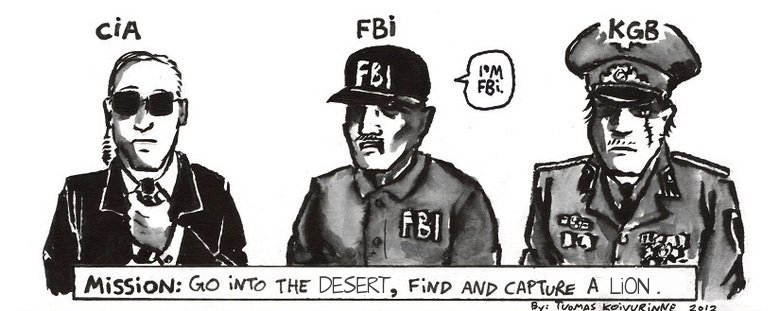
\includegraphics[width=0.5\textwidth]{img/loewenjagd.png}
		\end{figure}
	\end{outputbox}
	
	\Code
	\begin{lstlisting}
Man fange was man finde und prügele sie solange, bis sie zugibt, ein Löwe zu sein, der in der Wüste gefangen wurde.
\begin{figure}
	\centering
	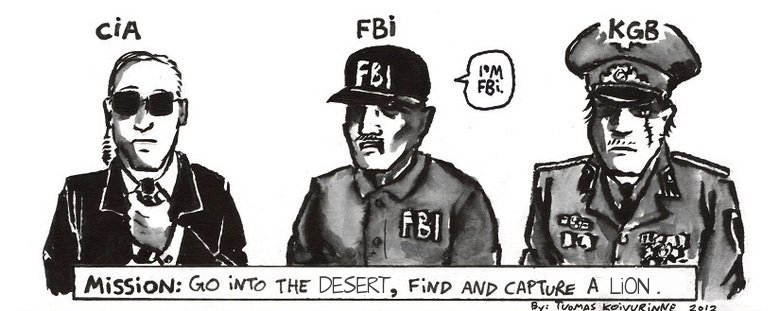
\includegraphics[width=0.5\textwidth]{img/loewenjagd.png}
\end{figure}
	\end{lstlisting}
\end{frame}
%%-----------------------------------------------------------------------------------------------%
%%------------------------------------------SUBSECTION-------------------------------------------%
%%-----------------------------------------------------------------------------------------------%
\subsection{Bildunter- und -überschriften}
\begin{frame}[c]
	\begin{center}
		\large Bildunter- und -überschriften
	\end{center}
\end{frame}
%-----------------------------------------------------------------------------------%
%---------------------------------------FRAME---------------------------------------%
%-----------------------------------------------------------------------------------%
\begin{frame}[fragile]
	\begin{Aufgabe}
		Füge eine Bild\textbf{unter}schrift mit dem Text
		
		\textrm{\qquote{Vergleich verschiedener Dienste bei der Löwenjagd.}}
		
		ein.
	\end{Aufgabe}

	\btVFill\Befehle
	\begin{center}
		\begin{tabular}{ll}
			\toprule
			\LaTeX\ Befehl								&	Funktion								\\ \midrule
			\lstinline|\includegraphics[]{}|			&	Befehl zum Einbinden von Grafiken		\\ 
			\lstinline|\centering|						&	Zentrierung								\\
			\lstinline|\begin{figure}...\end{figure}|	&	Umgebung für Abbildungen				\\
			\lstinline|\caption{}|						&	Text der Bild Unter- oder Überschrift	\\
			\lstinline|\textwidth|						&	Gibt die Breite des Textbereichs aus	\\
			\bottomrule
		\end{tabular}
	\end{center}
	\vspace{0.1cm}
\end{frame}
%-----------------------------------------------------------------------------------%
%---------------------------------------FRAME---------------------------------------%
%-----------------------------------------------------------------------------------%
\begin{frame}[fragile]
	\Losung
	\begin{outputbox}
		Man fange was man finde und prügele sie solange, bis sie zugibt, ein Löwe zu sein, der in der Wüste gefangen wurde.
		\begin{figure}
			\centering
			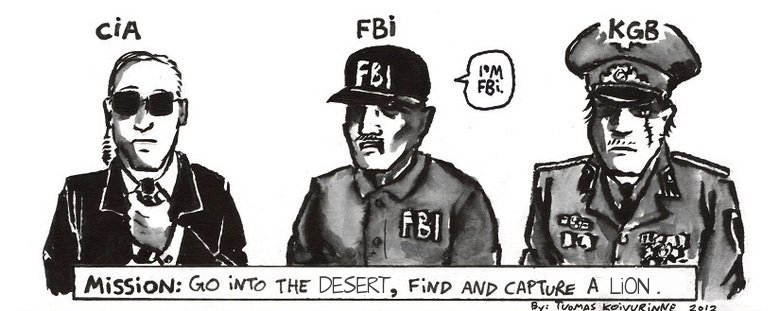
\includegraphics[width=0.1\textwidth]{img/loewenjagd.png}
		\end{figure}
		\begin{center}
			\textbf{Abbildung 1} - \textit{Vergleich verschiedener Dienste bei der Löwenjagd.}
		\end{center}
	\end{outputbox}

	\Code
	\begin{lstlisting}
Man fange was man finde und prügele sie solange, bis sie zugibt, ein Löwe zu sein, der in der Wüste gefangen wurde.
\begin{figure}
	\centering
	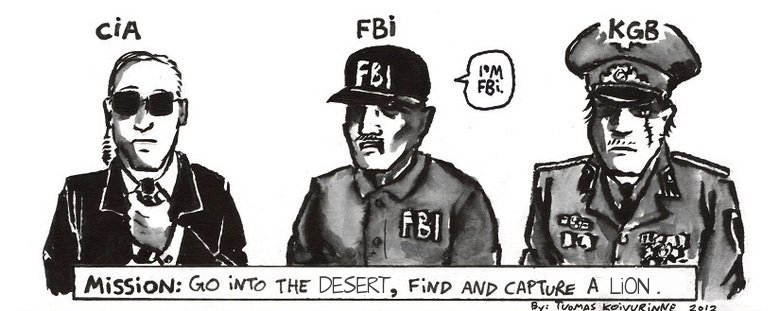
\includegraphics[width=0.1\textwidth]{img/loewenjagd.png}
	\caption{Vergleich verschiedener Dienste bei der Löwenjagd.}
\end{figure}
	\end{lstlisting}
\end{frame}